% typical processing for PostScript (PS) output:
%
%  latex advanced_example
%  bibtex advanced_example  (bibliography)
%  makeindex -s nomencl.ist -o advanced_example.gls advanced_example.glo
%                            (nomenclature)
%  latex advanced_example   (repeat as needed to resolve references)
%
%  xdvi advanced_example    (onscreen draft display)
%  dvips advanced_example   (postscript)
%  gv advanced_example.ps   (onscreen display)
%  lpr advanced_example.ps  (hardcopy)
%
% With the above, only Encapsulated PostScript (EPS) images can be used.
%
% Typical processing for Portable Document Format (PDF) output:
%
%  pdflatex advanced_example
%  bibtex advanced_example    (bibliography)
%  makeindex -s nomencl.ist -o advanced_example.gls advanced_example.glo
%                              (nomenclature)
%  pdflatex advanced_example  (repeat as needed to resolve references)
%
%  acroread advanced_example.pdf  (onscreen display)
%
% If you have EPS figures, you will need to use the epstopdf script
% to convert them to PDF because PDF is a limited subset of EPS.
% pdflatex accepts a variety of other image formats such as JPG, TIFF,
% PNG, and so forth -- check the documentation for your version.
%
% If you do *not* specify suffixes when using the graphicx package's
% \includegraphics command, latex and pdflatex will automatically select
% the appropriate figure format from those available.  This allows you
% to produce PS and PDF output from the same LaTeX source file.
%
% To generate a large format (e.g., 11"x17") PostScript copy for editing
% purposes, use
%
%  dvips -x 1467 -O -0.65in,0.85in -t tabloid advanced_example
%
% For further details and support, read the User��s Manual, aiaa.pdf.



\documentclass[]{aiaa-tc}% insert '[draft]' option to show overfull boxes

 \usepackage{varioref}%  smart page, figure, table, and equation referencing
 \usepackage{wrapfig}%   wrap figures/tables in text (i.e., Di Vinci style)
 \usepackage{threeparttable}% tables with footnotes
 \usepackage{dcolumn}%   decimal-aligned tabular math columns
  \newcolumntype{d}{D{.}{.}{-1}}
 \usepackage{nomencl}%   nomenclature generation via makeindex
  \makeglossary
 \usepackage{subfigure}% subcaptions for subfigures
 \usepackage{subfigmat}% matrices of similar subfigures, aka small multiples
 \usepackage{fancyvrb}%  extended verbatim environments
  \fvset{fontsize=\footnotesize,xleftmargin=2em}
 \usepackage{lettrine}%  dropped capital letter at beginning of paragraph
 \usepackage[dvips]{dropping}% alternative dropped capital package
 \usepackage[colorlinks]{hyperref}%  hyperlinks [must be loaded after dropping]


%%%%% Title %%%%%
 \title{Multi-species Fluid Flow Simulations using a Hybrid Computational Fluid Dynamics - Molecular Dynamics Approach 
% \skonote{Or "Polyatomic Lagrangian Dynamics Modeling for a Hybrid Computational Fluid Dynamics - Molecular Dynamics Approach"} 
}
%%%%% End Title %%%%%


%%%%% Author %%%%%
 \author{
  Nayong Kim\thanks{An IT Consultant; Center for Computation \& Technology,
  Louisiana State University, Baton Rouge, LA 70803, USA; Non-AIAA Member}\\
  {\normalsize\itshape
   Louisiana State University, Baton Rouge, USA}\\
  \and
  Soon-Heum Ko\thanks{A Computational Scientist; National Supercomputing Centre,
  Link\"{o}ping University, Link\"{o}ping, 581 83 Sweden; AIAA Member 450100;
  Corresponding Author}\\
  {\normalsize\itshape
   Link\"{o}ping University, Link\"{o}ping, Sweden}\\
  \and
  Shantenu Jha\thanks{An Assistant Professor; Department of Electrical and Computer Engineering,
  94 Brett Road, Piscataway, NJ 08854, USA; Non-AIAA Member}\\
  {\normalsize\itshape
   Rutgers University, Piscataway, USA}\\
  \and
  Brian Novak\thanks{A Post-doctoral Researcher; Department of Mechanical Engineering,
  Louisiana State University, Baton Rouge, LA 70803, USA; Non-AIAA Member}
    \ ,
  Dorel Moldovan\thanks{An Associate Professor; Department of Mechanical Engineering,
  Louisiana State University, Baton Rouge, LA 70803, USA; Non-AIAA Member}
    \  and
  Dimitris E. Nikitopoulos\thanks{A Professor; Department of Mechanical Engineering,
  Louisiana State University, Baton Rouge, LA 70803, USA; AIAA Member}\\
  {\normalsize\itshape
   Louisiana State University, Baton Rouge, USA}\\
 }
%%%%% End Author %%%%%


 % Data used by 'handcarry' option
 \AIAApapernumber{YEAR-NUMBER}
 \AIAAconference{Conference Name, Date, and Location}
 \AIAAcopyright{\AIAAcopyrightD{YEAR}}

 % Define commands to assure consistent treatment throughout document
 \newcommand{\eqnref}[1]{(\ref{#1})}
 \newcommand{\class}[1]{\texttt{#1}}
 \newcommand{\package}[1]{\texttt{#1}}
 \newcommand{\file}[1]{\texttt{#1}}
 \newcommand{\BibTeX}{\textsc{Bib}\TeX}


%%%%% Note Configuration %%%%%
\newcommand{\jhanote}[1]{ {\textcolor{red} { ***Jha: #1 }}}
\newcommand{\nynote}[1]{ {\textcolor{blue} { ***NKim: #1 }}}
\newcommand{\skonote}[1]{ {\textcolor{green} { ***Jeff: #1 }}}
\newcommand{\menote}[1]{ {\textcolor{purple} { ***Comment from ME: #1 }}} 
%%%%% End Note Configuration %%%%%


\begin{document}

\maketitle


%%%%% Abstract %%%%%
\begin{abstract}
The constrained Lagrangian dynamics modeling in the hybrid computational fluid dynamics (CFD) - molecular dynamics (MD) approach is improved for the simulation of multi-species polyatomic fluid.
%\Microscopic mean velocity term on the classical Lagrangian dynamics equation is replaced by the division of mean linear momentum and mean mass to account for multi-species fluid system.
The primitive formulation of the classical Lagrangian dynamics equation is replaced by conservative form to account for multi-species fluid system.
Also, the equation is applied on molecules instead of individual atom, to preserve the linear momentum between continuum and particle domain without encountering the unfavorable numerical break-down of molecular bonding.
We verify our hybrid CFD-MD simulation package by analyzing a nano-scale transient Couette flow of a single monatomic fluid.
The multi-species polyatomic Lagrangian dynamics modeling has been evaluated by analyzing two different fluid models: the mixture of two monatomic fluids and a polyatomic molecular fluid under the short-range potential.
These two applications verify the accuracy of the proposed model and
evaluate the hybrid CFD-MD approach as a tool to describe the complex
flow field near the solid obstacle.
\end{abstract}
%%%%% End Abstract %%%%%


%\printglossary %creates nomenclature section produced by MakeIndex


%%%%% Introduction %%%%%
\section{Introduction}
\label{sec:intro}

\lettrine[nindent=0pt]{T}{he} hybrid computational fluid dynamics (CFD) - 
molecular dynamics (MD) approach is getting more attraction as a potential 
answer in describing the nano-scale flow phenomena. In this approach,
the fluid system is divided into subdomains and individual subdomain is
solved by either the continuum solver or the particle-based solver.
Conventionally, the macroscopic flow region where the continuum hypothesis is
valid is resolved by the continuum formulation and the material interface 
(e.g. fluid/solid or fluid/fluid) is analyzed by higher degree-of-freedom 
particle formulation. Compared with the classical CFD or MD methodology, 
this approach is expected to provide the high-resolution solution near 
the wall boundary within the acceptable computational cost.

A number of scientific studies have been published which improve the hybrid
technique and/or apply this approach to various nano-scale flow fields.
These researches can be categorized to constrained Lagrangian dynamics
\cite{Thompson,Nie,Yen,Liu,ECCOMAS10}, alternating 
Schwarz method\cite{Hadjicon2,Hadjicon3,Werder}, 
and direct flux exchange\cite{Flekkoy,Delgado1,Time_Mechanism,Giupponi},
according to the formulation of hybrid schemes and the characteristics of 
variables exchanged in the overlapping region. Of these methods, the 
constrained Lagrangian dynamics applies the constrained Lagrangian dynamics
equation to impose the hybrid MD boundary condition. Continuum and particle
solvers exchange density properties (i.e., conservative variables) 
and they are coupled in time space. Compared to other counterparts, this
method is easy to implement, is directly applicable to the unsteady flow 
simulation, and its molecular samples are less noisy than the flux properties.


%\lettrine[nindent=0pt]{T}{he} hybrid computational fluid dynamics (CFD) - 
%molecular dynamics (MD) approach is getting more attraction as a potential 
%answer in accurately describing the nano-scale flow phenomena within 
%the acceptable computational cost. A number of scientific studies have been
%published using this approach, which can be categorized to constrained 
%Lagrangian dynamics~\cite{Thompson,Nie,Nie_cavity,Cui,Wang,Yen,Liu,AJK2011}, 
%alternating Schwarz method~\cite{Hadjicon1,Hadjicon2,Hadjicon3,Werder,Kotsalis}, 
%and direct flux exchange~\cite{Flekkoy,Wagner,Delgado1,USHER,Time_Mechanism,Giupponi}.
%Of these methods, the constrained Lagrangian dynamics is easy to implement, 
%is directly applicable to the unsteady flow simulation, and molecular sample is
%less noisy than the flux-based approach.


Meanwhile, this approach is only valid for the single-species monatomic fluid 
flow since the constrained Lagrangian dynamics equation does not consider
the mass variation of fluid particles. So, the direct application of the classical
constrained Lagrangian dynamics equation to multi-species fluid domain results in
the break-up of momentum conservation. Also, the application to the polyatomic fluid
whose atomic mass are different ends up with the numerical break-up of chemical bond.

This motivates us to refine the classical constrained Lagrangian dynamics equation
for the application to multi-species and polyatomic fluid flow. The equation is
reformulated to provide the linear momentum conservation. Also, the equation is
applied on the molecules instead of individual atoms, to prevent the numerical
break-up of chemical bond. We implement this equation on our hybrid CFD-MD simulation
package which has been introduced in our previous article\cite{ECCOMAS10} and apply
it to solving multi-species and polyatomic fluid flow.

We introduce the hybrid CFD-MD approach and describe the Lagrangian dynamics equation
for multi-species polyatomic fluid particles in Section~\ref{sec:hybrid}. Numerical
methods and the hybrid interface on individual solvers are addressed in Section
\ref{sec:numerics}. Section~\ref{sec:result} is dedicated to present 
numerical solutions of the transient Couette flow in different fluid systems.
The first system consists of two monatomic fluids whose chemical properties are
equivalent to the liquid argon with the variation in mass. The next one contains
the polyatomic molecules whose molecular structure is water (hydrogen oxide)
while the long-range interaction is not considered. We 
summarize our studies and propose further applications in Section~\ref{sec:conclusion}.
%%%%% End Introduction %%%%%


%%%%% Hybrid Schema %%%%%
\section{Hybrid CFD-MD Approach for Multi-species Polyatomic Fluid}
\label{sec:hybrid}

\subsection{The Hybrid CFD-MD Approach}
\label{sec:hybrid_design}


%%%%% FIGURE %%%%%
\begin{wrapfigure}{R}{0.5\linewidth}
%\includegraphics{Hybrid_Schematic.pdf}
\includegraphics{Hybrid_Schematic.jpg}
\caption{Schematic Diagram of the Hybrid Domain with Detailed View of Overlapping Zone: 
Left figure expresses the composition of hybrid simulation domain and 
the right figure presents individual layers in the overlapping region.}
\label{Fig:Couette}
\end{wrapfigure}
%\begin{figure}
%\centering
%\includegraphics[width=0.5\linewidth]{Hybrid_Schematic.pdf}
%\caption{Schematic Diagram of the Hybrid Domain with Detailed View of Overlapping Zone: 
%Left figure expresses the composition of hybrid simulation domain and 
%the right figure presents individual layers in the overlapping region.}
%\label{Fig:Couette}
%\end{figure}
%%%%% FIGURE %%%%%


A detailed structure of the fluid domain for the hybrid CFD-MD approach is
described in Figure~\ref{Fig:Couette}. CFD solves the flow region where 
the continuum hypothesis is valid while MD analyzes the complex microscopic 
flow feature near the solid obstacle. Overlapping region is placed sufficiently 
far from the solid stationary wall to prevent the direct influence of 
molecular-level physics.

The overlapping region is designed sufficiently large to contain 
five individual layers with sufficient spacing. From the bottom, 
we have the {\it{particle-to-continuum}} and {\it{continuum-to-particle}} 
(denoted as 'MDtoCFD' and 'CFDtoMD', respectively) layers where hybrid
boundary condition for CFD and MD are imposed. The external force layer
for particle systems is placed on the top (farthest from the
material interface) of the overlapping region. These three ''active'' layers 
are separated by the buffer layer, which is designed to prevent direct 
interaction between particles in above ''active'' layers.

Hybrid CFD boundary condition on MDtoCFD layer is imposed by averaging
molecular properties located in this layer. This boundary condition is prone to
suffer from the statistical error\cite{Hadjicon3,Time_Mechanism}, since
the finite number of particles participate in sampling process in space and time.
Therefore, the delicate determination of coupling parameters are very important
for acquiring the noise-free hybrid solution. The distance from the material 
interface and the size of sampling layer determines the scale of statistical 
error in space; how long the molecular properties will be accumulated
(''sampling duration'') and how often these samples are applied to the 
continuum solver (''sampling interval'') also affects the sampling noise in time.

The hybrid MD boundary condition is imposed by referencing the continuum solution
in this layer. A single set of continuum solution is imposed to higher
degree-of-freedom molecular domain through the constrained Lagrangian dynamics
equation. This equation constrains particles to attain the macroscopic flow property 
(conservative properties) on average, while preserving their degree-of-freedom of 
translational motion. Details on this equation will be presented in Section
\ref{sec:hybrid_multispecies}.

In the uppermost layer, a fictitious external force is exerted on particles 
to preserve the system ensembles of the particle domain. This force function
is designed to be short-range so as not to influence the motion of the particles 
past the buffer layer in the CFDtoMD domain. The force stiffens as the particles 
approach outer region to prevent the particles from drifting out of the 
particle domain. We apply a cost-effective classical external force model 
by Nie {\it{et al.}}\cite{Nie}. 


\subsection{Constrained Lagrangian Dynamics for Multi-species Fluid Simulation}
\label{sec:hybrid_multispecies}


Once the hybrid simulation accomplished for the monatomic system, it was developing for the more realistic problem, which is multi-species polyatomic fluids including water molecules. The first step of the development was start with modifying to the equation of motion in coupling CFDtoMD region\cite{Nie}. The average velocity of particles in J{\it{th}} cell is equal to the velocity $\it u_J$ in continuum cell, and it can be depicted as eq. ~\ref{eq:gov1} with taking Lagrangian derivative.

%\begin{equation}
% u_{J}(t) = \frac{1}{N_{J}} \displaystyle\sum_{k} v_{k} =  {  \frac{\displaystyle\sum_{k}m_{k}\  {\dot x_k(t)}} {\displaystyle\sum_{k}m_{k}}}
% \label{eq:Con_vel}
%\end{equation}
%\normalsize
%where $\it v_{k}$ is the velocity of $\it k^{th}$ particle and $\it N_{J}$ is the number of particles in the cell, and $\it m_{k}$ is the mass of $\it k^{th}$ particle.  With taking Lagrangian derivative of eq. ~\ref{eq:Con_vel},

\vspace{-.2em}
%\footnotesize
\begin{equation}
% \frac{Du_{J}(t)}{Dt} = {  \frac{\displaystyle\sum_{k}m_{k}\  \frac{d\dot x_k(t)}{dt} } {\displaystyle\sum_{k}m_{k}}} = {  \frac{\displaystyle\sum_{k}m_{k}\  {\ddot x_k(t)}} {\displaystyle\sum_{k}m_{k}}}
  \frac{Du_{J}(t)}{Dt} = {  \frac{\displaystyle\sum_{k}m_{k}\  \frac{d\dot x_k(t)}{dt} } {\displaystyle\sum_{k}m_{k}}} 
 \label{eq:gov1}
\end{equation}
\normalsize
where $\it v_{k}$ is the velocity of $\it k^{th}$ particle and $\it N_{J}$ is the number of particles in the cell, and $\it m_{k}$ is the mass of $\it k^{th}$ particle. 

The Classical MD equation of motion can be generalized to obtain the constraint by adopting the fluctuation in the acceleration of each particles, $\zeta_{k}$

\vspace{-.2em}
%\footnotesize
\begin{equation}
\frac{F_{k}}{m_{k}}  =  \ddot{x_{k}}(t) =  \frac{Du_{J}(t)}{Dt} + \zeta_{k} = {  \frac{\displaystyle\sum_{k}m_{k}\  {\ddot x_k(t)}} {\displaystyle\sum_{k}m_{k}}}+ \zeta_{k} =  {  \frac{\displaystyle\sum_{k}F_{k}(t)} {\displaystyle\sum_{k}m_{k}}}+ \zeta_{k}
 \label{eq:zeta1}
\end{equation}

\begin{equation}
\zeta_{k} = \ddot{x_{k}}(t) - {  \frac{\displaystyle\sum_{k}F_{k}(t)} {\displaystyle\sum_{k}m_{k}}}= \frac{F_{k}(t)}{m_{k}} - {  \frac{\displaystyle\sum_{k}F_{k}(t)} {\displaystyle\sum_{k}m_{k}}} 
 \label{eq:zeta2}
\end{equation}
\normalsize
where $\zeta_{k}$ is  a variance on each particles adequate to  \begin{equation}{\displaystyle\sum_{k}m_k\zeta_{k} = 0}\end{equation} and $m_k$  = $m$ only for monatomic system. 

Finally, constrained particle dynamics equation was modified with the conventional equation of motion considering multi-mass to simulate polyatomic CFD-MD coupling hybrid simulation, it can be written as:
\vspace{-.2em}
%\footnotesize
\begin{equation}
 \ddot{x_{k}}(t) = \frac{F_{k}}{m_{k}} -  \frac{1}{m_k} \frac{\displaystyle\sum_{i=1}^{N_J}F_{i}} {\displaystyle\sum_{i=1}^{N_J}m_{i}} - \frac{m_k}{\Delta t_{MD}} \{  \frac{\displaystyle\sum_{i=1}^{N_J}m_{i}\dot{x_{i}}} {\displaystyle\sum_{i=1}^{N_J}m_{i}} - u_{J}(t + \Delta t_{MD})\}
 \label{eq:EOM}
\end{equation}
\normalsize

The forces on the cell caused by particle interactions with other particles are revised with averaged force and velocity in the cell and informed velocities from CFD computation. The acceleration of the cell is now constrained instead of the average acceleration of the particle in the cells in this equation.  Again, these two quantities are the same when all of the masses of atoms are the same. 


%1. How classical constrained Lagrangian dynamics equation is implemented

%-- what is the objective: to eventually equilibrate the continuum and mean microscopic velocity

%-- what is the governing equation: the governing equation and the meaning of each term under the equation

%2. Why it needs change

%-- The limitation of the equation to be applied to multi-species fluid model

%3. How it is improved

%-- The formulation of "Polyatomic Multi-species Constrained Lagrangian Dynamics Equation"

%-- Difference compared to the original equation

%-- Difference in applying the equation: apply on the center of mass of each molecule, not on individual atom (which will imply that atoms under the same molecule will experience the same acceleration, which tells that the linear momentum is of particular concern)

%%%%% End Hybrid Schema %%%%%


%%%%% Numerical Schemes %%%%%
\section{Development of a Hybrid CFD-MD Simulation Package}
\label{sec:numerics}

We address the numerical schemes and hybrid interface of individual CFD and MD
solvers in brief: More details can be found in Ref.~\citen{ECCOMAS10}.

\subsection{Continuum Incompressible Flow Solver}
\label{sec:numerics_cfd}

The current in-house continuum hydrodynamics code solves the unsteady 
incompressible Navier-Stokes equations. In this work, the pseudo-compressibility 
method\cite{PseudoCompressibility} is adopted to form a hyperbolic system of 
equations which can be marched in pseudo-time.
For time-accurate unsteady simulation, a dual time stepping method is adopted 
and it is combined with the LU-SGS (Lower-Upper Symmetric Gauss-Seidel) scheme
\cite{LU-SGS} for the implicit time integration. The inviscid fluxes are 
upwind-differenced using Osher's flux-difference splitting scheme\cite{Osher}. 
For higher-order spatial accuracy, the MUSCL (Monotone Upstream-centered 
Schemes for Conservation Laws)\cite{MUSCL} approach is used on the inviscid 
flux calculation. Viscous fluxes are calculated using conventional 
second-order central differencing.


%The current in-house continuum hydrodynamics code solves the unsteady 
%incompressible Navier-Stokes equations: 

%\vspace{-.2em}
%\begin{eqnarray}
%\frac{\partial {u}_{i}}{\partial {x}_{i}} = 0
%\end{eqnarray}
%\vskip-.6cm
%\begin{eqnarray}
%\frac{\partial {u}_{i}}{\partial t} + \frac {\partial} {\partial {x}_{j}} ({u}_{i}{u}_{j}) = -\frac {\partial p} {\partial {x}_{i}} + \nu \frac {{\partial}^2 {u}_{i}} {{\partial} {x}_{j} \partial {x}_{j}} \nonumber
%\end{eqnarray}
%where $\nu$ is the kinematic viscosity.

%In this work, the pseudo-compressibility method\cite{PseudoCompressibility} 
%is adopted to form a hyperbolic system of equations which can be marched 
%in pseudo-time.
%A time derivative of pressure is added to the continuity equation resulting in

%\vspace{-.2em}
%\begin{eqnarray}
%\frac{\partial (p/\rho)}{\partial \tau} = - \beta \frac{\partial {u}_{i}}{\partial {x}_{i}}
%\end{eqnarray}
%where $\beta$ denotes a pseudo-compressibility parameter, currently set up to 2.5.

%For time-accurate unsteady simulation, a dual time stepping method is adopted 
%and it is combined with the LU-SGS (Lower-Upper Symmetric Gauss-Seidel) scheme
%\cite{LU-SGS} for the implicit time integration. The inviscid fluxes are 
%upwind-differenced using Osher's flux-difference splitting scheme\cite{Osher}. 
%For higher-order spatial accuracy, the MUSCL (Monotone Upstream-centered 
%Schemes for Conservation Laws)\cite{MUSCL} approach is used on the inviscid 
%flux calculation. Viscous fluxes are calculated using conventional 
%second-order central differencing.


\subsection{Particle Dynamics Solver}
\label{sec:numerics_md}

Newton's conservation of momentum is employed at the atomic level to propagate 
the system's motion through time evolution. In this work the most commonly used 
Lennard-Jones (12-6) intermolecular force potential model\cite{Allen} is employed 
to calculate pair-wise interactions of particles in the system. A cut-off distance
is introduced to reduce the computational cost and is set to be 2.2 magnitude of
atomic characteristic length\cite{Travis}. The most common velocity Verlet 
algorithm\cite{Allen} is employed for time integration of the equations of motion 
of the interacting particles and to compute molecular trajectories in the simulation.
In this work, the MD simulations were performed by using an appropriately 
modified version of the Large Atomic Molecular Massively Parallel Simulator 
(LAMMPS). It is a classical molecular dynamics open-source code written in C++ 
and developed by Sandia National Labs\cite{LAMMPS_url}.

%In MD, an initial velocity is assigned to each atom, and Newton's conservation 
%of momentum is employed at the atomic level to propagate the system's motion 
%through time evolution. In this work the most commonly used Lennard-Jones 
%(12-6) intermolecular force potential model is employed to calculate pair-wise 
%interactions of particles in the system, and is defined as:

%\vspace{-.2em}
%\begin{equation}
% u(|r_{i} - r_{j}|) = 4\epsilon_{ij}[(\frac{\sigma_{ij}}{r_{ij}})^{12}-(\frac{\sigma_{ij}}{r_{ij}})^{6}]
% \label{eq:LJ12}
%\end{equation}
%\normalsize

%where  $\epsilon_{ij}$ and $\sigma_{ij}$ denote the pair-wise potential well 
%depth and the atom size parameter respectively, and $r_{ij}$ is the distance between 
%the particle i and j. The repulsive term $\it 1/r_{ij}^{12}$ dominating at 
%short $r_{ij}$ distance is based on the Pauli principle to avoid 
%overlapping the electronic clouds when particles are very close to each other. 
%The attractive term $\it 1/r_{ij}^{6}$ dominates at long range representing 
%Van der Waals dispersion forces. A cut-off distance $\sigma_{c}$ is introduced 
%here to reduce the computational cost and is set to be 2.2$\sigma$\cite{Travis}.
%Namely when $r_{ij}$ exceeds the cutoff the intermolecular force is set to zero 
%without being calculated.

%The most common velocity Verlet algorithm is employed for time integration 
%of the equations of motion of the interacting particles and to compute molecular 
%trajectories in the simulation.

%In this work, the MD simulations were performed by using an appropriately 
%modified version of the Large Atomic Molecular Massively Parallel Simulator 
%(LAMMPS). It is a classical molecular dynamics open-source code written in C++ 
%and developed by Sandia National Labs~\cite{LAMMPS_url}.


\subsection{Implementation of Hybrid Schemes and Interface}
\label{sec:numerics_hybrid}


The file-based communicator is implemented on each solver to exchange conservative
properties at every sampling interval. CFD solver stores the instantaneous solution
at that time instance, while MD solver produces the backward sample over the
sampling duration. Thus, transferred boundary information is extrapolated along
the temporal space so as to avoid the time-lagging pattern in the boundary.
CFD solver directly applies these extrapolated properties as the 
hybrid boundary condition at each time instance. MD solver inputs these values
on employed constrained Lagrangian dynamics formulation. MD solver also applies the external force function in the uppermost layer.

The unit conversion function is also incorporated in CFD solver. This function changes
the non-dimensional CFD solution into non-dimensional MD unit and vice versa. 
Considering the current formulation of CFD solver, the artificial pressure property
needs to be converted to an equivalent molecular mass density. We acquire the relation
between artificial compressibility {\it{P}} and density $\rho$ by comparing 
the mass conservation equation and artificial compressibility formulation:

\begin{equation}
\frac{\partial P}{\partial t} = {a}^2 \frac{1}{\rho} \frac{\partial \rho}{\partial t}
\label{eq:Ar_Co1}
\end{equation}

This relation, written in discretized form, provides the hybrid number density
and/or artificial pressure boundary conditions. CFD solutions in the hybrid 
MD boundary layer is rewritten in density form as,

\begin{equation}
\rho_{N+1} = \frac{\rho_{N}}{1 - \frac{P_{N+1} - P_{N}}{a^2}}
\label{eq:Ar_Co2}
\end{equation}

Likewise, sampled molecular density is converted to equivalent artificial pressure
at the hybrid CFD boundary layer as,

\begin{equation}
P_{N+1} = P_{N} + a^2 ( 1 - \frac{\rho_{N}}{\rho_{N+1}} )
\label{eq:Ar_Co3}
\end{equation}

From above equations, {\it{a}} denotes the artificial speed of sound and {\it{N}},
{\it{N+1}} stands for the time step.

Coupling parameters, such as location and size of hybrid layers in space and 
sampling interval and sampling duration in time, are delicately determined 
by the reference to previous studies\cite{Nie,Yen,Liu,Hadjicon2,Werder,Flekkoy,Delgado1}
and preliminary measurement of noise level on pure molecular dynamic domain.
We also apply the replica sampling approach\cite{REMD} in case the individual 
hybrid solution suffers from the excessive sampling noise. This approach averages 
multiple independent simulations from the different initial Maxwell-Boltzmann 
distribution to find the non-fluctuating solution. The solution from N replicas 
provide the same order of accuracy as an individual solution from N times larger 
domain: this approach (running multiple small tasks instead of one big task) is 
computationally more effective in view of scheduling on many supercomputing
resources.


%%%%% Numerical Solutions %%%%%
\section{Numerical Results}
\label{sec:result}

\subsection{Problem Description and Validation}
\label{sec:result_val}

The application problem is a transient Couette flow problem, which is widely used
for the verification of the hybrid CFD-MD solver. Fluid model is the liquid argon, whose
characteristic length is ${\sigma}=3.405{\times}10^{-10}$ meter and the time scale is 
$\tau=2.2{\times}10^{-12}$ second. The number density is $0.81m{\sigma}^{-3}$.
The channel is 52 $\sigma$ in height and the solid wall has artificial properties 
that are the same as those of liquid argon. The slip ratio between the fluid and the wall
material is set at 0.6 to satisfy the linear velocity gradient along a vertical 
direction.~\cite{Nie}



The computational domain for the hybrid simulation is depicted in Figure
\ref{Fig:Couette_Val_Domain}. The pure MD region is specified as 10 $\sigma$, 
that was reported to be sufficient to prevent the excessive sampling noise
on the hybrid CFD boundary condition.\cite{Yen} Individual hybrid layer has
2 $\sigma$ in height. Hybrid CFD boundary region consists of two consecutive 
layers to provide the accurate boundary condition for this collocated mesh system.
The width of the MD domain along the periodic direction is determined at 140 
$\sigma$, after a number of numerical experiments.
Both the sampling interval and the sampling duration are set to be 10 $\tau$,
considering the characteristics of our deterministic application targets. 

%%%%% FIGURE %%%%%
\begin{figure}[ht]
\centering
\begin{minipage}[b]{0.45\linewidth}
\centering
%\includegraphics{Couette_Val_Domain.pdf}
\includegraphics{Couette_Val_Domain.jpg}
\caption{Computational Domain of the Couette Flow Simulation: The height 
of the fluid domain is 52$\sigma$ ($\approx$177$\AA$). CFD mesh size is 
71$\times$27 and CFD cells at the pure MD region are treated as holes. 
MD domain size is about 140$\sigma$ along the horizontal direction and 
around 26$\sigma$ along the vertical direction, including the bottom wall. 
Periodic boundary condition is applied on the principal flow direction.}
\label{Fig:Couette_Val_Domain}
\end{minipage}
\hspace{0.5cm}
\begin{minipage}[b]{0.45\linewidth}
\centering
%\includegraphics{Flat_Plate_Sol2.pdf}
\includegraphics{Flat_Plate_Sol2.jpg}
\caption{A Time-accurate Couette Flow Profile:
The evolution of velocity field along the vertical direction is presented.
CFD solution is the instantaneous profile at specified time and
MD solution is spatially averaged over 2 $\sigma$ in height and
temporally averaged for 1 sampling durations (=10$\tau$).
Hybrid solution presents the same flow physics as the analytic solution
with the slight variation due to the sampling noise.}
\label{Fig:Flat_Plate_Sol}
\end{minipage}
\end{figure}
%%%%% FIGURE %%%%%




%%%%% FIGURE %%%%%
%\begin{wrapfigure}{L}{0.45\linewidth}
%%\includegraphics{Couette_Val_Domain.pdf}
%\includegraphics{Couette_Val_Domain.jpg}
%\caption{Computational Domain of the Couette Flow Simulation: The height 
%of the fluid domain is 52$\sigma$ ($\approx$177$\AA$). CFD mesh size is 
%71$\times$27 and CFD cells at the pure MD region are treated as holes. 
%MD domain size is about 140$\sigma$ along the horizontal direction and 
%around 26$\sigma$ along the vertical direction, including the bottom wall. 
%Periodic boundary condition is applied on the principal flow direction.}
%\label{Fig:Couette_Val_Domain}
%\end{wrapfigure}
%%%%% FIGURE %%%%%


%%%%% FIGURE %%%%%
%\begin{wrapfigure}{R}{0.45\linewidth}
%%\includegraphics{Flat_Plate_Sol2.pdf}
%\includegraphics{Flat_Plate_Sol2.jpg}
%\caption{A Time-accurate Couette Flow Profile: The evolution of velocity field 
%along the vertical direction is presented. CFD solution is the instantaneous 
%profile at specified time and MD solution is spatially averaged over 
%2 $\sigma$ in height and temporally averaged for 1 sampling durations (=10$\tau$).
%Hybrid solution presents the same flow physics as the analytic solution
%with the slight variation due to the sampling noise.}
%\label{Fig:Flat_Plate_Sol}
%\end{wrapfigure}
%%%%% FIGURE %%%%%


Figure~\ref{Fig:Flat_Plate_Sol} presents a transient Couette flow profile 
by the hybrid simulation which is compared to the analytic solution. 
The hybrid solution succeeds in describing the same flow physics as the 
analytic solution under the level of molecular dynamic sampling noise.
This evaluates the accuracy of the current hybrid simulation package
as a tool for solving the nano-scale flow field. This sampling noise is 
even diminished further through the sampling of multiple replicas.


%\begin{figure}
%\centering
%\begin{subfigmatrix}{2}
%\subfigure[Analytic Solution, Pure CFD and MD Results]{\includegraphics[width=0.4\linewidth]{Flat_Plate_Sol1.pdf}}
%\subfigure[Pure CFD and Hybrid Simulations]{\includegraphics[width=0.4\linewidth]{Flat_Plate_Sol2.pdf}}
%\end{subfigmatrix}
%\caption{A Time-accurate Couette Flow Profile: The evolution of velocity field 
%along the vertical direction is presented. CFD solution is the instantaneous 
%profile at specified time and MD solution is spatially averaged over 
%2 $\sigma$ in height and temporally averaged for 1 sampling durations (=10$\tau$).
%Hybrid solution presents the same flow physics as the analytic solution
%under the sampling noise level.}
%\label{Fig:Flat_Plate_Sol}
%\end{figure}


%Figure~\ref{Fig:Flat_Plate_Sol} presents a transient Couette flow profile 
%by CFD, MD, and hybrid simulations. Solution by the CFD is identical to the
%analytic solution and an MD simulation also describe the same flow physics
%while a slight fluctuation due to the sampling noise is also observed. 
%The hybrid solution also describes the same flow physics as the analytic 
%solution under the same magnitude of the sampling noise as the pure MD result.
%This sampling noise is even diminished further through the sampling of
%multiple replicas.\cite{JoCS2012}


\subsection{Transient Couette Flow Profiles in Multi-species and Polyatomic Fluids}
\label{sec:result_multi}

We apply our simulation package to solving a liquid compound which consists of
two monatomic molecule species varying in mass. Atomic properties 
are numerically designed to be equivalent to the above liquid argon system,
except the mass of individual particle. The systematic density and
total number of particles are still the same as the above validation problem, 
so as to provide the reliability on preserving other characteristic properties.

We simulated two different composition of particles to verify
the constrained Lagrangian dynamic equation for multi-species fluid.
The first system consists of two molecular species whose non-dimensional
mass (compared to that of a liquid argon) are 0.5 and 1.5, respectively.
Same number of particles are mixed to compose a fluid domain.
The second system contains two species with 0.4 and 4.0 non-dimensional
molecular mass whose ratio of particle numbers are 5:1.

Figure~\ref{Fig:Multi_species} presents the transient Couette flow profile
of each problem. In comparison to the analytic solution, both simulations
show the same flow evolution. It verifies the accuracy of the multi-species
Lagrangian dynamics model. Hybrid steady-state solutions at time of
1500 $\tau$ shows a little faster velocity than the analytic solution.
This difference is due to the slight slip of liquid particles near the
solid obstacle, as is also observed in the pure molecular dynamic simulation
in Fig.~\ref{Fig:MD_Multi_species}.
The molecular dynamic simulation is capable of detecting this "natural"
wall-slip phenomenon according to the inter-molecular characteristc
energy. On the other hand, empirical boundary condition modelings are 
necessary to describe the same flow physics from pure CFD simulations.
This evaluates the strength of the hybrid simulation as a way of accurately
describing the complex flow pattern near the solid boundary interface.
%Also, the time-lagging profile during the evolution is presented. This is
%related to the accuracy of the temporal coupling scheme. It motivates us
%to refine the time integration method.


%%%%% FIGURE %%%%%
%\begin{wrapfigure}{R}{1.0\linewidth}
\begin{figure}
 \begin{subfigmatrix}{2}% number of columns
  \subfigure[Mixture of 0.5 and 1.5 Mass Atoms]
  {{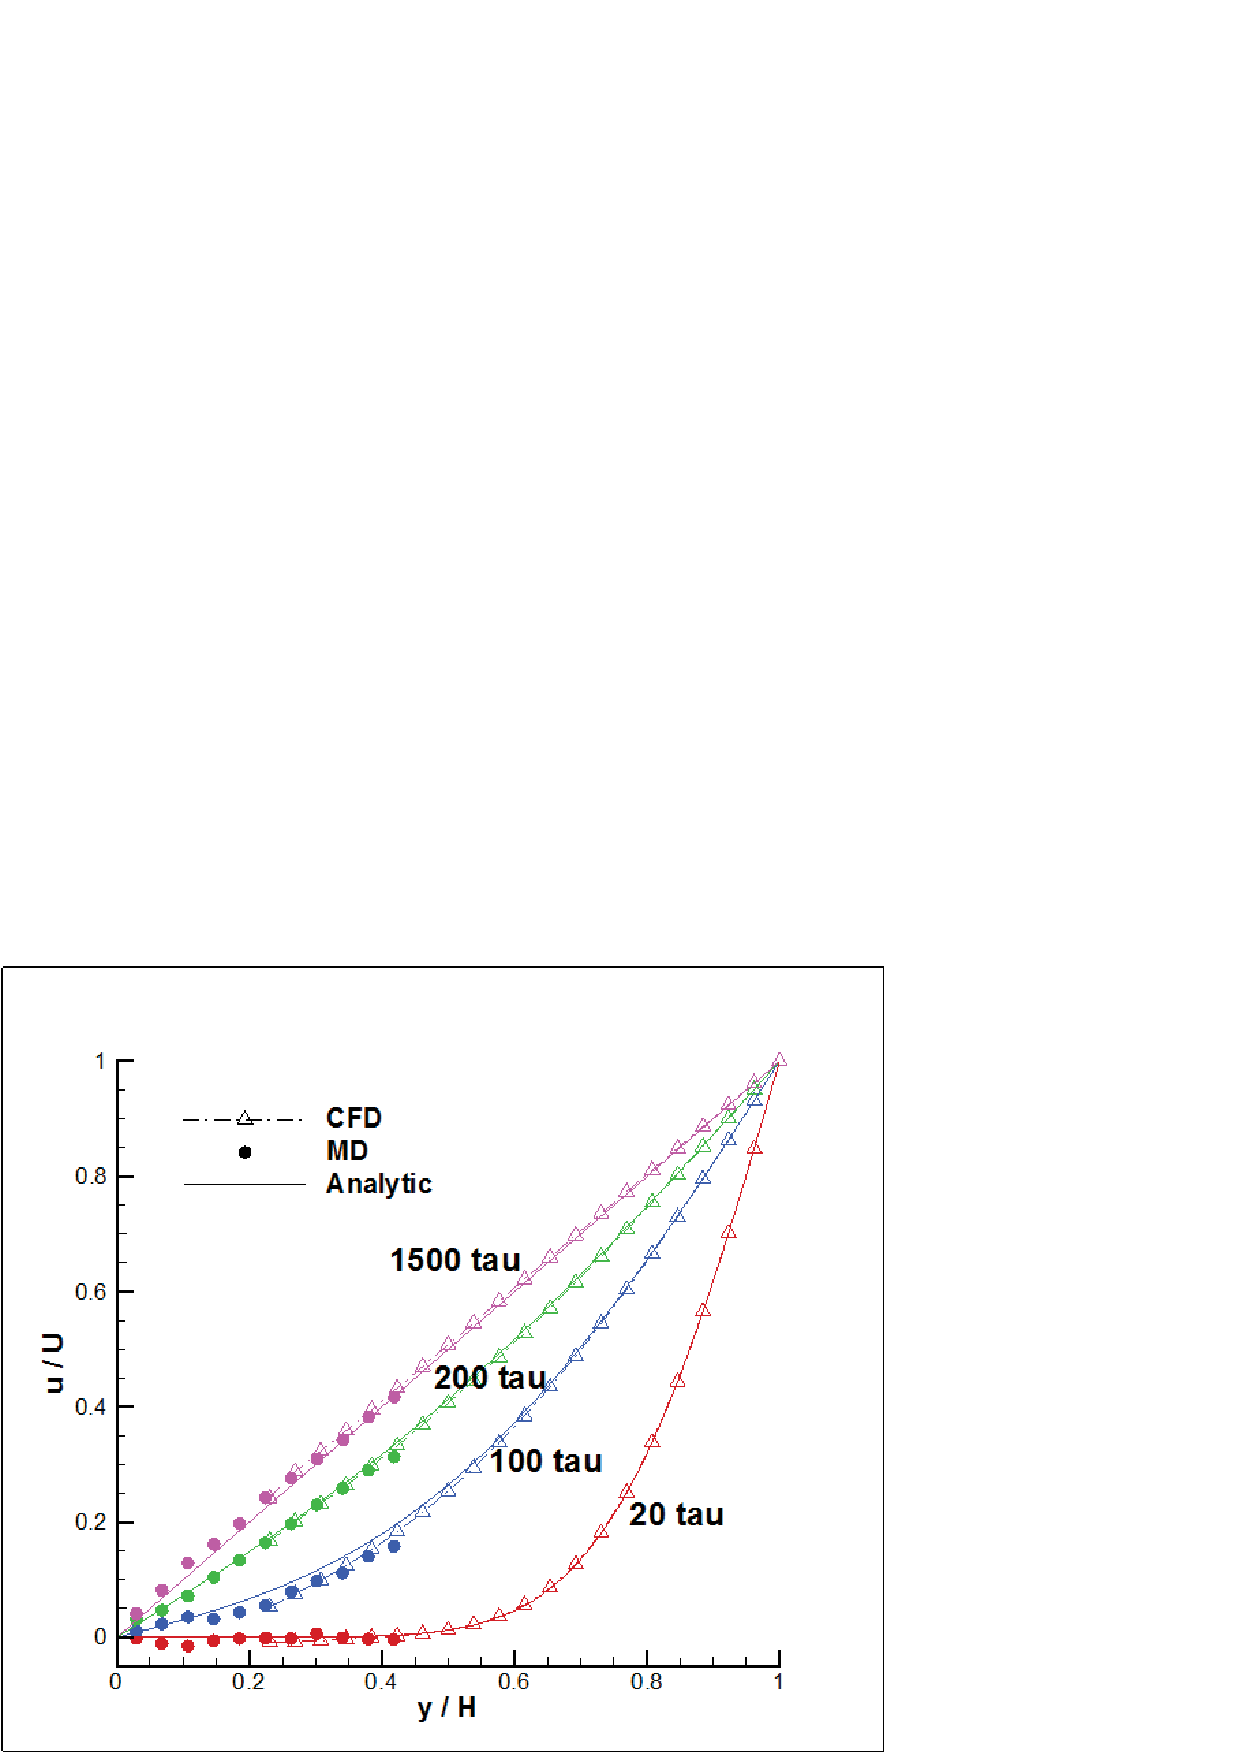
\includegraphics{050150.jpg}}{\label{050150}}}
  \subfigure[Mixture of 0.4 and 4.0 Mass Atoms]
  {{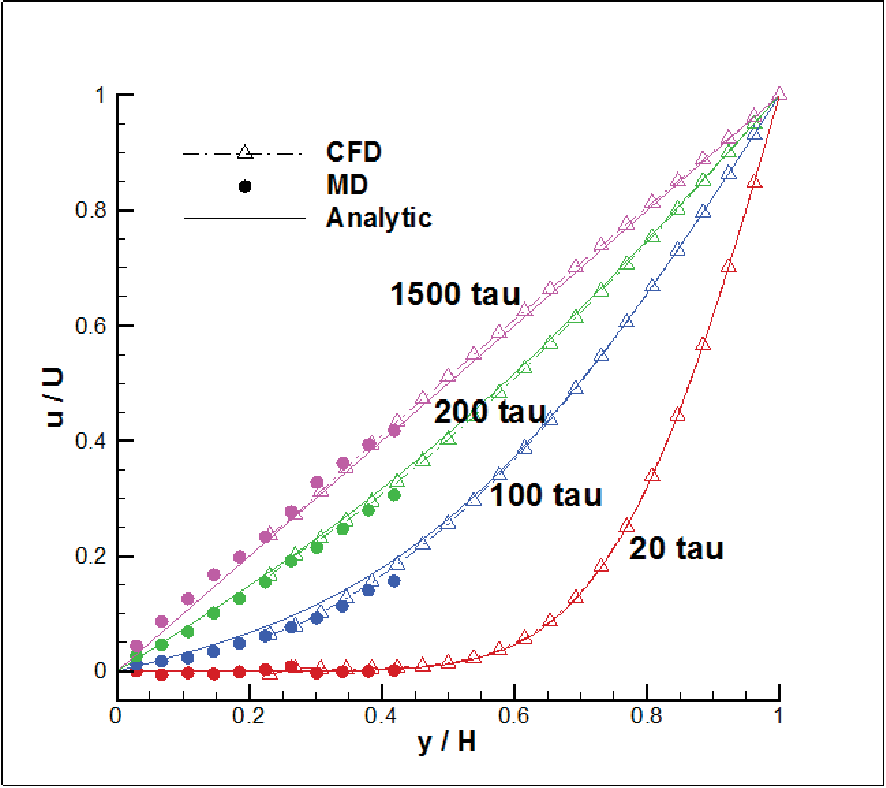
\includegraphics{040400.jpg}}{\label{040400}}}
 \end{subfigmatrix}
 \caption{Couette Flow Profiles in Multi-species Liquids:
 Time-variant velocity profile along the vertical direction are presented.
 Both simulations from different particle compositions accurately describe
 the flow physics, which verifies the multi-species Lagrangian dyanmics
 model.}
 \label{Fig:Multi_species}
\end{figure}
%\end{wrapfigure}
%%%%% FIGURE %%%%%


%%%%% FIGURE %%%%%
%\begin{wrapfigure}{R}{1.0\linewidth}
\begin{figure}
 \begin{subfigmatrix}{2}% number of columns
  \subfigure[Steady-state Couette Flow Profile via a Pure MD Simulation]
  {{\includegraphics{040400_PureMD.jpg}}{\label{PureMD}}}
  \subfigure[Hybrid and Pure MD Results near the Bottom Wall]
  {{\includegraphics{040400_PureMD_Closer.jpg}}{\label{Near_Wall}}}
 \end{subfigmatrix}
 \caption{Couette Flow Simulation by the Pure Molecular Dynamics:
 A mixture of 0.4 -- 4.0 non-dimensional mass particles has been simulated.
 Buth pure MD and hybrid simulations describe the physical phenomenon of
 wall-slip in response to the inter-molecular characteristic energy
 between solid and liquid particles. Pure MD and hybrid results slightly
 differ far-from-the-wall region, due to different imposition of upper
 wall boundary condition (natural slip by particle-based method VS
 non-slip condition in continuum approach).}
 \label{Fig:MD_Multi_species}
\end{figure}
%\end{wrapfigure}
%%%%% FIGURE %%%%%


The next experiment solves the polyatomic molecular fluid whose
molecular structure is that of water, i.e., density is 9.98 $kg/m^{3}$ and
viscosity is 3.0$\times$$10^{-4}$$kg/(m\cdot{s})$. Domain size and
flow conditions are the same as the above validation problem, also is
the hybrid layer configuration. CFD and MD simulations exchange
hybrid boundary conditions at every 20 pico seconds. In the MD simulation,
the bottom wall material is the disordered Lennard-Jones carbon and
6771 fluid molecules participate in flow simulation. The Coulombic interaction
has been computed for a short-range (up to 8 ${\AA}$ in distance from
individual atom), due to the impossibility of accounting for
the Coulombic effect from CFD region.


%%%%% FIGURE %%%%%
\begin{wrapfigure}{R}{0.5\linewidth}
%\begin{figure}
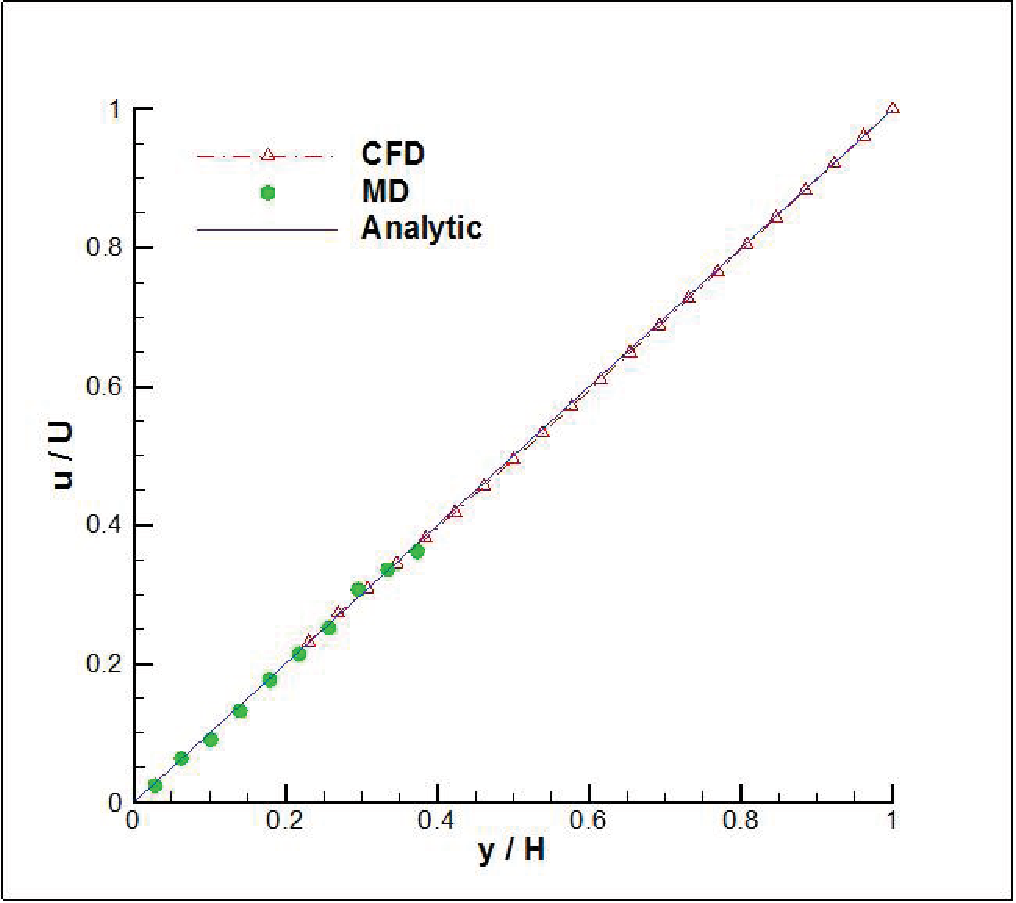
\includegraphics{Water_Steady.jpg}
\caption{Steady-State Couette Flow Profile of Water:
 The hybrid solution averaged over 200 pico seconds is compared with
 the analytic solution. The close agreement between two solutions
 verify the accuracy of the constrained Lagranging dynamics modeling
 for polyatomic molecules.}
\label{Fig:Water}
%\end{figure}
\end{wrapfigure}
%%%%% FIGURE %%%%%


The steady-state hybrid solution is presented in Fig.~\ref{Fig:Water}.
The result matches well with the analytic solution. It proves that
the proposed constrained Lagrangian dynamics modeling is capable of
solving the polyatomic molecules without harming the molecular structure.
The visualized result is the averaged solution over 200 pico seconds
(from 2600 to 2800 pico seconds) after the flow reached the steady-state.
The instantaneous profile is highly fluctuative due to the molecular
brownian motion, which is resolved as the number of molecular sample
increases.
Meanwhile, increasing the MD problem size will result in the excessive
request on computing power: even the current simulation runs one full day
with 256 CPU cores at one of most powerful supercomputers (Ranger in
Texas Advanced Computing Center\cite{Ranger}). It necessitates
the design of numerical models to suppress the statistical noise of
molecular samples.

%%%%% End Numerical Solutions %%%%%



%%%%% Conclusion and Future Works %%%%%
\section{Conclusion and Future Works}
\label{sec:conclusion}

We have proposed the improved constrained Lagrangian dynamics model for 
a hybrid CFD-MD simulation in this paper. It is designed to satisfy 
the momentum conservation of the fluid solution and avoid the numerical
instability in applying the equation to polyatomic molecules. The 
classical constrained Lagrangian dynamics equation is reformulated
to satisfy the linear momentum conservation of the multi-species fluid
system and the equation is applied on the center of mass of each 
molecule to preserve the chemical bond of a polyatomic molecule.
We have implemented this model on our hybrid CFD-MD simulation package
which consists of a pseudo-compressibility incompressible Navier-Stokes
solver and a molecular dynamics solver solving the Lennard-Jones
potential. The simulation package has been verified by solving the 
transient Couette flow profile of a single-species monatomic fluid 
system. We have applied our simulation package to solving the multi-species
monatomic fluid. Simulations at different composition of particles
present accurate solutions compared to the analytic solution, which verify
the multi-species Lagrangian dynamics equation.
Also, the simulation of a polyatomic fluid provides
the numerical validity of imposing the constrained Lagrangian dynamics
equation on molecular level. These numerical experiments, in turn,
expresses the potential to apply the hybrid CFD-MD approach to any fluid
systems.

The future work will be dedicated to modeling the effect of
long-range interaction in hybrid simulation. Up to now, hybrid simulations
fail to consider the long-range potentials since outside the hybrid region
is modeled as the vacuum in view of particle domain. Mathematically
modeling the long-range force field or putting the virtual slab 
on the border of hybrid region could be ones of potential answers.

%%%%% End Conclusion and Future Works %%%%%


%%%%% Acknowledgement %%%%%
\section*{Acknowledgement}

This work has been accomplished as a part of the Cybertools
(http://cybertools.loni.org) project which was primarily funded by 
NSF/LEQSF (2007-10)-CyberRII-01. 

%Content

%%%%% End Acknowledgement %%%%%


% produces the bibliography section when processed by BibTeX
\bibliography{Bibs/Hybrid}
\bibliographystyle{aiaa}

\end{document}

% - Release $Name:  $ -

